\section{Results}
\label{sec:results}

The primary experiment is the Class~A search for a drifting, unresolved
spectral carrier: \NWinA{} fine-channel windows toward \NSysClassA{}
systems. The Class~B search for an unresolved spectral excess is secondary
and carries no drift discrimination: \NWinB{} coarse windows. Together they
are the \NWindows{} windows of the primary census. \textbf{No event
satisfied the confirmation criterion set out in \S\ref{sec:summary}.} What
follows is first how deep the search reaches, and then what it found and how
each finding was disposed of.

\subsection{Sensitivity: the power at which a carrier would have been
found} \label{sec:pninetysel}

\emph{The sensitivity of this survey is a recovery completeness of one epoch,
and not a threshold.} Artificial carriers were injected at a random
sub-channel phase and a random drift from each window's own grid and recovered
through the unchanged pipeline; the power at which nine in ten come back is
$\mathrm{EIRP}_{90}$, the only sensitivity quoted here, and what it measures
is recovery through the single-epoch trigger stage --- the trigger and the
localisation at the stellar position, inside one execution block.
\textbf{It is therefore the power at which a
carrier would have produced a crossing and not the power at which one would
have been confirmed}, because confirmation needs a second and separated epoch,
which the archive supplies for some systems and not others whatever their
depth (\S\ref{sec:confirmability}). The \NCtrl-position spatial rank decides
nothing and is not charged against it either: charging it would cost a further
factor $\SensCostLike$ and in \SensNRingHiUnres{} bright-ring windows could not
be met at any injected power (Fig.~\ref{fig:strata}).

\emph{Measured that way the completeness is one number for the class.} Nine
carriers in ten are recovered at $\EirpNinetyMultA\,P_{\rm trig}$; the sampling
error of that pooled value is $\pm\SensBootPct$ per cent, which is a statement
about the class average and about no individual window. Every one of the
\SensNInj{} directly injected Class~A windows resolves a ninety per cent point
of its own, and the value does not depend on the brightness of its control
ring: the \SensNRingHi{} windows whose ring carries resolved emission come
back at $\SensRingHi\,P_{\rm trig}$ against $\SensRingLo$ for the rest
(Fig.~\ref{fig:strata}). Class~B carries
its own factor $\EirpNinetyMultB\,P_{\rm trig}$, measured the same way from
\SensNToneCoarse{} carriers injected into \SensNInjCoarse{} coarse windows of
\SensNInjCoarseBlock{} execution blocks; it is what sets the limits for
Barnard's Star, Wolf~359 and Proxima.

\emph{The resulting limits.} The median Class~A window reaches
$\EirpNinetyWinMedA$\,W of equivalent isotropic radiated power and the median
system, on its best window, $\EirpNinetySysMedA$\,W, with a spread across
systems of $\EirpNinetySysLoA$--$\EirpNinetySysHiA$\,W
(Fig.~\ref{fig:classasens}a). The round $10^{15}$\,W level is reached for
\NSysEfifteen{} of them. The calibration of the factor is good to
$\times\SensFacLo$--$\times\SensFacHi$ (Table~\ref{tab:p90budget}); that is
the interval on the median and on the counts, and not on any one window's
limit. One bias is not inside it and runs one way only: an injected carrier is
added to already calibrated visibilities and so suffers no atmospheric
decorrelation, whereas a real carrier does. Measured block by block from the
phase rms the observatory records on each block's phase calibrator
\citep[\S10.4.9]{ALMAHandbook}, through the standard phase-scatter relation
\citep[Eq.~3]{Richards2022}, it leaves the median limit optimistic by
\SensDecorPct{} per cent and the median window above \SensDecorHiGHz{}\,GHz by
\SensDecorHiPct{} per cent, so the limits at the top of the frequency range
are the least secure quoted here.

\emph{Two further losses act window by window, and both are divided out of
the limits above rather than quoted beside them.} The search's phase centre
omits the annual parallax, which displaces the star by a median
\SensBeamsMed{} of a synthesised beam and at most \SensBeamsMax; dividing by
the amplitude a compact source retains there
(Appendix~\ref{app:conventions}) makes the median Class~A limit shallower by
\PxaShiftWinPct{} per cent, and \PxaMissingStar{} in \PxaMissingEb{} has no
astrometric keys and is left uncorrected. The second loss the injections do
not reproduce at all, because each injected carrier is laid down at one
frequency per integration while a real one sweeps within it, keeping
$\mathrm{sinc}(\pi\Delta/2)$ of its peak amplitude for an excursion of
$\Delta$ channels. At the drift that sets a ninety per cent point this comes
from each window's own integration length for \SmcNMeas{} of the \NWindows{}
windows and is bounded at \SmcDtCeil\,s for the rest.
\textbf{It costs nothing in the median window and up to $\times\SmcFacWorst$
in the \SmcNAbove{} finest-channel ones, which are also the deepest}: the best
Class~A window moves from $\SmcWinLoWas$ to $\EirpNinetyWinLoA$\,W, and
\SmcLostStars{} drops out of the \SmcSysEfifteenWas{} systems that would
otherwise reach $10^{15}$\,W.

\emph{Carriers were injected directly into \SensNInj{} of the \NWinA{}
Class~A windows, \SensNInjPct{} per cent, and the result transferred to the
remaining \SensNTransfer, which is the dominant caveat on all of the above.}
The injected windows are the Class~A windows of execution blocks drawn in a
stratified random order fixed in advance and without reference to which
windows hold a crossing; they hold \SensNCrossAch{} crossings against the
\SensNCrossExp{} the population rate predicts. \emph{The unit is the block and
not the window}, because a block's calibrated visibilities are what an
injection campaign has to rebuild: the draw controlled band and array, and
channel width, ring brightness and integration length matched the population
afterwards to \SensCovWorstPct{} per cent on the worst axis.

\textbf{A window that was not injected therefore carries an estimated
$\mathrm{EIRP}_{90}$}, and across the injected windows the ninety per cent
point ranges from $\times\SensIndivFacLo$ to $\times\SensIndivFacHi$ of the
adopted factor: that dispersion, not the calibration interval above, is what
one uninjected window's own limit is uncertain by. Because a system's limit is
its best window, a minimum over several such estimates could favour windows
whose own factor falls below the class average; drawing each window's factor
from the \SensNInj{} measured ones instead, over \ScRsNTrial{} trials, moves
the per-system median deeper by \ScRsMedShiftPct{} per cent, holds the count
at $10^{15}$\,W to \ScRsNLo--\ScRsNHi{} in nine trials in ten, and spreads one
system's own limit by $-\ScRsSysLoPct$ to $+\ScRsSysHiPct$ per cent, so the
estimate is mildly conservative and the statistics formed over the class are
unaffected. But \textbf{the best window was itself injected into for only
\SmcNMeasSys{} of the \NSysClassA{} systems}: for the other \SmcNEstSys{} the
headline limit is an estimate.

\emph{A carrier that is not always radiating is penalised in proportion.} The
de-drifted stack is coherent across a whole execution block, so a carrier
present for a fraction of one comes back at that fraction of its continuous
amplitude. Over \DutyNTrial{} trials at duty cycles down to
\DutyCycleMinPct{} per cent the recovered amplitude followed the duty cycle to
\DutyAttenDevPct{} per cent, so a transmitter radiating a tenth of the time
needs $\DutyPowFac\times$ the power quoted above; those trials carry no drift,
so the joint drifting and intermittent case is not measured here.

\begin{table}
\centering
\scriptsize
\caption{What sets $\mathrm{EIRP}_{90}$, and in which direction. The
uncertainty on the calibration is an uncertainty on the class-average factor,
and so on any statistic formed over many windows; the flux term within it is
band-dependent, so the submillimetre windows carry the larger of the two
combined figures. The spread between windows
is an observed dispersion and is the statement about one window's own limit;
the signed terms are biases, stated with their direction rather than folded
into an error bar. The decorrelation bias is measured in \SensDecorNBlk{} of
the \SensDecorNBlkTot{} execution blocks, those whose delivery records the
phase stability, and is not imputed to the rest.}
\label{tab:p90budget}
\tiny
\setlength{\tabcolsep}{2pt}
% GENERATED by sens_r11.py -- do not hand-edit.
\begin{tabular}{@{}l@{~~}r@{~~}>{\raggedright\arraybackslash}p{0.37\columnwidth}@{}}
\hline
 & value & what it does to the limit \\
\hline
Class-average completeness & $\times3.03$ & nine carriers in ten recovered at this multiple of a window's own trigger power. \emph{Measured} in the 49 Class~A windows injected directly and \emph{estimated}, at this factor, in the other 353 \\
\hline
\multicolumn{3}{@{}l}{\emph{Uncertainty on that calibration} (per cent), combined in quadrature} \\
The factor itself & $\pm2$ & sampling error of the pooled value over the 49 injected windows \\
Absolute flux scale & $\pm\BudFlux$ & the observatory's own band-dependent specification (\BudFluxSource): \BudFluxSpec, weighted over this sample's bands \\
Distance and visibility scale & $\pm\BudDistVis$ & the Gaia parallaxes, which enter as $d^{2}$, and the block-to-block visibility scale \\
\emph{Combined} & $-11/+11$ & $\times0.89$--$\times1.11$ on the factor, and so on the median limit and on the system counts; $\pm\BudCombWorst$ for the \BudNHiWin{} Class~A windows in \BudHiBandWord~\BudHiBands, at \BudHiGHzList\,GHz \\
\hline
\multicolumn{3}{@{}l}{\emph{Spread between windows}. An observed dispersion, not an error bar.} \\
Window to window & $\times0.80$--$\times1.58$ & the 49 injected windows resolve 2.41--4.80\,$P_{\rm trig}$ individually. This, and not the interval above, is what an estimated limit is uncertain by; it is wider, and it applies to \SmcNEstSys{} of the \NSysClassA{} systems \\
\hline
\multicolumn{3}{@{}l}{\emph{Applied}. Folded into every limit quoted, and so not combined with the above.} \\
Intra-integration smearing & $\times1.00$--$\times\SmcFacWorst$ & a carrier sweeps through part of a channel within one integration and the injected ones do not: $\eta_{\rm smear}$ at the drift that sets a ninety per cent point, from each window's own integration length where it is recorded (\SmcNMeas{} windows) and from the longest delivered anywhere where it is not (\SmcNBound) \\
Annual parallax & $\times1.00$--$\times2.06$ & the phase centre omits it, so each limit is divided by the amplitude a compact source retains at its own displacement, a median \PxaLossMedPct\,per cent \\
\hline
\multicolumn{3}{@{}l}{\emph{Signed terms}. A bias is not an error bar and is not added to one.} \\
Channel response & $\times\InjPeakAtNinety$ & carried by the injections, so already inside the completeness above \\
\quad its residual & $+\InjShortPct$ & the injected profile falls short of the exact response: \emph{conservative} \\
Primary-beam model & $+0/+10$ & ALMA's beamwidth in place of the pipeline's Airy-null one: nothing in the median window, 4 windows of one star \\
Decorrelation & $+0/+\SensDecorPct$ & measured block by block from the phase rms the observatory records on each block's phase calibrator, which an injected carrier does not suffer and a real one does: $+\SensDecorHiPct$ above \SensDecorHiGHz\,GHz, and more than $+\SensDecorTailLevelPct$ in \SensDecorTailPct{} per cent of windows \\
\hline
\end{tabular}

\end{table}

\begin{figure}
\centering
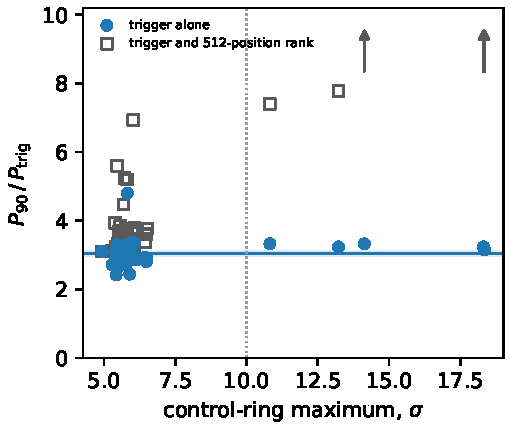
\includegraphics[width=0.96\columnwidth]{figures/sens_ring.pdf}
\caption{Why one completeness factor serves the whole class. Each of the
\SensNInj{} of the \NWinA{} Class~A windows that were injected directly is
plotted at the power that recovers nine carriers in ten, against the
maximum of its own
\NCtrl-position control ring. Filled circles are the criterion adopted
here --- the trigger and localisation at the star --- with the pooled value
and its uncertainty as the line and band; they show no trend with the ring.
Open squares add the demand that the carrier outrank every control position,
and arrows mark the windows that then reach ninety per cent at no injected
power. Dotted, the $\SensRingRule\sigma$ ring brightness above which a ring
carries resolved emission rather than noise.}
\label{fig:strata}
\end{figure}

\begin{figure*}
\centering
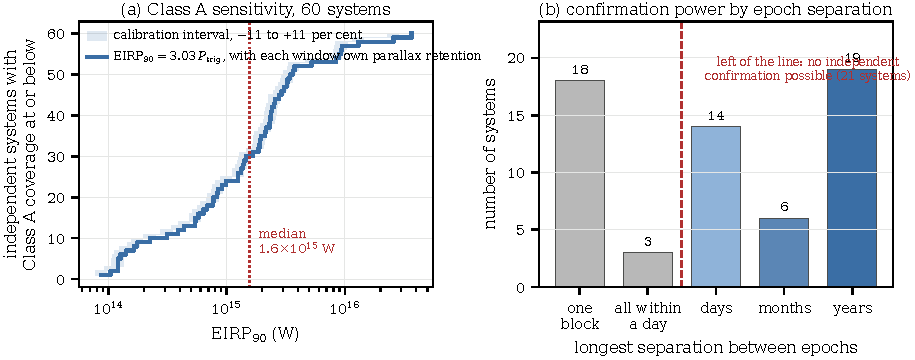
\includegraphics[width=0.92\textwidth]{figures/classa_sensitivity.pdf}
\caption{\textbf{The two completenesses of the carrier search, over the same
\NSysClassA{} systems.} \emph{(a)}~Single-epoch trigger completeness: the
cumulative number of systems whose best window reaches a given
$\mathrm{EIRP}_{90}$, the power at which nine carriers in ten produce a
crossing at the star inside one execution block, on the one adopted convention
$\EirpNinetyMultA\,P_{\rm trig}$ with each window's own annual-parallax retention
applied; the shaded band is the calibration interval of
Table~\ref{tab:p90budget}. \emph{(b)}~Confirmation completeness, which no
amount of power buys: systems grouped by the longest separation between their
searched epochs, more than \EpSep{} day counting as independent. \textbf{For
the \ScSysOneBlock{} observed in a single block and the \ScSysSameDay{} whose
blocks all fall within one day --- left of the dashed line, \ScSysNoConf{}
systems --- confirmation was not possible at any sensitivity in panel~(a)}:
what panel~(a) gives them is a crossing limit, not a detection limit.}
\label{fig:classasens}
\end{figure*}

\subsection{The nearest stars: Barnard's Star and Wolf~359}
\label{sec:barnardswolf}

Barnard's Star is the second-nearest stellar system and Wolf~359 the third if
brown dwarfs are excluded, and to our knowledge these are the first millimetre
or submillimetre technosignature limits for either \citep{Enriquez2017,
Price2020, Margot2023}. Both are non-detections. \emph{Both limits come from
the secondary Class~B experiment and not from the carrier search}: the archive
holds only coarse Band~6 windows toward these stars, so what is constrained is
an unresolved spectral excess and not a drifting carrier. On the
$\mathrm{EIRP}_{90}$ convention of \S\ref{sec:pninetysel} Barnard's Star
reaches $\EirpNinetyBarnLo$--$\EirpNinetyBarnHi$\,W over \NWinBarn{} windows
and Wolf~359 $\EirpNinetyWolfLo$--$\EirpNinetyWolfHi$\,W over \NWinWolf.

\subsection{Threshold crossings and how each was disposed of}
\label{sec:technosearch}

\emph{The result is a chain of three tests, and it is read in one direction.}
Of the windows the search covers --- the \NWindows{} of the primary census
and the archival-tail blocks beside them --- \EvNCrossRaw{} hold a cell
reaching $T\geq5$ at the stellar position. \EvNCrossFlag{} lie in the one
execution block that fails the quality criterion of \S\ref{sec:bdblock}, fixed
before it was applied, so the population that characterises the search is the
\EvNCrossQp{} in quality-passing data and those \EvNCrossFlag{} are reported
beside it. The molecular-line mask, $\pm\MaskHalfKms$\,km\,s$^{-1}$ wide in
each star's own rest frame, places \MkNCoinc{} of the \EvNCrossQp{} within
that distance of a catalogued transition; \MkNSODecideWord{} of those
coincidences are with a species no debris disc has been shown to carry and are
reported rather than acted on (Appendix~\ref{app:linemask}), leaving
\EvNAttrQp{} attributed and \EvNUnattrQp{} unattributed. The attributions are
kinematic and not an accident of bandwidth: \AppMTubeObs{} of the
\AppMNCrossF{} crossings with a measured peak frequency fall within
$\pm\DispoHalfKms$\,km\,s$^{-1}$ of a searched transition, against
\AppMTubeNull{} expected were each peak free to land anywhere on its own
window's grid (Appendix~\ref{app:rfi}). Of the unattributed,
\EvNRankQp{} outrank all \NCtrl{} control positions of their own window, and
none was found again in any later epoch covering its frequency. \textbf{No
crossing survives the chain, and this survey reports no detection.}
Figure~\ref{fig:chain} counts what survives each step and
Tables~\ref{tab:ledger} and~\ref{tab:ledgercont} list every crossing.

\emph{Anything bright in a window hides a weaker carrier behind it, so the
weaker cells were sought too.} The retained statistic is the de-drifted value
in every channel, so a window may hold several crossings, neighbouring
channels above the trigger counting as one. Over the \CkNWin{} Class~A windows
whose per-channel statistic survives --- the \CkNWinNotCov{} that do not hold
\CkRegMiss{} crossings between them --- the \CkNPrimary{} primary crossings
are accompanied by
\CkNSecondaryWord{} secondary ones, in \CkNSecWin{} windows and as many as
\CkNSecMax{} in one; \CkNSecAttr{} are the resolved carbon monoxide of a disc
spread over channels and \CkNSecUnattrWord{} are unattributed, toward
\CkSecStars. Each of those \CkNSecUnattrWord{} has \CkCovLo--\CkCovHi{}
covering blocks and \CkNRecurWord{} reaches the trigger in any of them, the
deepest repeat being $T_\star=\CkTrepHi$. Keeping only the window maxima
returns the \CkRegN{} tabulated crossings, at the published frequency to
\CkRegDev{} of a channel. Counting cells at the star means counting cells in
the controls, and outside the mask the star holds \CkRatioLo--\CkRatioHi{}
times as many as a control position at every level from $T=\CkLadderLo$ to the
trigger, with no step where a carrier search would put one; the expectation
that follows is \S\ref{sec:trigunif}'s. Requiring two neighbouring channels to
share a drift rate before counting as one would instead give \CkRuleSec{}
secondary crossings and \CkRuleSecUnattr{} unattributed, \CkRuleSplit{} of
them one excursion counted twice, and none of those recurs either.

\subsubsection{Most of the crossings are expected by chance}
\label{sec:trigunif}

The trigger is a threshold on a statistic and not a false-alarm rate: the
number of searched channel\,$\times$\,drift cells per window spans
\TuCellsDecades{} decades, so one level buys very unequal protection. How
many crossings chance should produce is therefore measured window by window,
over the \CeNWin{} Class~A windows of the census and with one condition on
both sides of the comparison: a cell at the stellar position that reaches the
trigger and that the line mask does not attribute. A window's own \NCtrl{}
control positions measure how often a position in that field reaches the
trigger, and the window's own channel grid measures how often such a position
would fall inside an attribution window, which takes \CeMaskPct{} per cent of
the total. The control positions differ from the star in one respect that
bears on this: they carry no continuum, so a calibration error that varied
with frequency would raise the star and not them. It cannot --- the stellar
continuum nowhere reaches \CdCnrMax{} times the single-channel noise, so an
error as large as the continuum itself would still fall short of the trigger
(Appendix~\ref{app:radius}). Chance predicts \CeExp{} unattributed Class~A
crossings, with \CeLo--\CeHi{} allowed by resampling the execution blocks the
windows come from, and \CeObs{} are found. Counting cells rather than windows
on both sides moves the two together: the same \CkNCtrlPos{} control positions
predict \CkExp{} cells, \CkExpSec{} of them beside a window's largest, against
\CkNObs{} and \CkNSecUnattr{} found and \CkLo--\CkHi{} allowed, because a
control position holds a second above-trigger cell about as often as a star
does (\S\ref{sec:technosearch}). A further \CeNTailCrossWord{} unattributed
crossings, both toward \CeTailStar, lie in archival-tail blocks the catalogue
does not tabulate window by window, and enter neither side.

The expectation is a sum of rates measured at control positions, and the
reserved blocks measure how far a star departs from them: carrying that
difference through moves it to \CeExpX, and the count agrees with chance
either way. The width of the range allowed is what the comparison can say and
no more --- an added population of as many as \CeAddBlind{} crossings would
sit inside it unremarked. What tests each crossing individually is the
recurrence test of \S\ref{sec:etacrv}.

\subsubsection{One execution block accounts for four of the crossings}
\label{sec:bdblock}

\BdNCross{} crossings belong to \BdStar{} (\BdAlias), all in one ACA execution
block, \texttt{\BdBlock}, whose whole field is above threshold:
\BdNCtrlAbove{} of \BdNCtrl{} control positions exceed $T=5$ against a survey
median control maximum of \BdSurvCtrlMed. Its single-integration noise is as
predicted (\BdRmsMeas\,Jy against \BdRmsPred\,Jy) but does not integrate down
--- a jackknife on the channel mean gives \BdJack\,Jy against
\BdThermal\,Jy thermal --- so a slow drift common to every channel and
position inflates the statistic across the field, while the \BdNSibling{}
sibling executions of the same field, array and setup reach only
$T_\star=\BdSibTMax{}$ and produce no crossing. \emph{What is inflated is the
field and not the star:} the strongest of the four reaches
$T_\star=\EvFlagTStarHi$ where its own controls peak at \EvFlagCtrlAtHi, and
\EvFlagNgeLo--\EvFlagNgeHi{} of the \BdNCtrl{} stand above the star. The
criterion fails this block and no other
(Appendix~\ref{sec:blockquality}), so its \BdNCross{} crossings are reported
apart from the \EvNCrossQp{}; Appendix~\ref{app:rfi} carries what the block
might instead be.

\subsubsection{Stellar flares are excluded by a broadband prediction}

The sample contains known flare stars. But a millimetre flare raises every
channel of a window alike, so one able to produce a single-channel crossing at
the trigger must produce a $5\sqrt{N}\sigma$ continuum event in the same
integrations. Over the \FlNCont{} crossings with a recoverable continuum
measurement that prediction runs \FlPredLo--\FlPredHi$\sigma$, against an
observed continuum statistic of median \FlObsMed{} with $|Z|<3$ in \FlNQuiet{}
of them. One block settles it: \FlEgStar{} \texttt{\FlEgEb} holds both a
crossing ($T_\star=\FlEgT$) and the millimetre flare of
\citet{MacGregor2020}, and \emph{that flare contributes \FlEgContrib$\sigma$
to the single-channel statistic} --- raising the continuum at $Z=\FlEgContZ$
while the crossing's own de-drifted track reaches $Z_{\max}=\FlEgTrackZ$.

\subsection{$\beta$~Pictoris: an astrophysical positive control, and the
obstacle it identifies} \label{sec:bpicval}

\emph{A search that finds nothing must show that it could have found
something, and the survey's strongest features show exactly that.} The
frozen pipeline recovers the $\beta$~Pictoris circumstellar carbon monoxide
blind, without being told the disc is there. It recovers it in two
rotational transitions and in \CsBpCoBlocks{} independent execution
blocks spanning \BpBaselineYr\,yr, and in \NStageOneBpicEb{} of those the
star also outranks every control: \BpicNFlagThree{} Band~3 windows at
$T_\star$ up to \BpicBThreeTsym, and \BpicNFlagSix{} Band~6 windows at
\BpicBSixTsym. The identification is kinematic and does not rest on those
statistics. Carried through the frame chain --- to the barycentre at each
block's own epoch, then to the star's rest frame --- all \BpicPanelNCo{}
crossings lie within \BpicDvCoHi\,km\,s$^{-1}$ of the stellar systemic
velocity, in the two lowest CO transitions of a star with mapped
circumstellar CO \citep{Dent2014,Matra2017}. The Band~3 peaks agree across blocks to
\BpRecThreeTuneChanMax{} channel once each block's own tuning is removed, so
any apparent drift is far below the grid searched. The alternative reading
requires a transmitter placed by coincidence at matched offsets from two CO
transitions of one star.

It is also the control that shows the recurrence test of
\S\ref{sec:etacrv} working in the positive direction: every flagged
$\beta$~Pictoris carbon-monoxide feature is recovered in an independent
execution block, the screened Band~6 window returning
$T_\star=\BpRecTTwo{}$ in the second block of its own recurrence set. A
non-recurrence elsewhere means nothing unless the same machinery recovers a
repeat where one exists.

\emph{One of those blocks is a counterexample, and it is the more useful half
of the control.} In it several of the \NCtrl{} control positions exceed the
stellar statistic, so the spatial rank disfavours a window holding carbon
monoxide known to be real and centred on the star; the disc is resolved on
the scale of the primary beam in that configuration, which is the geometry
the statistic is built to reject. The rank is therefore a test of
compactness and not of authenticity, and on a real extended source it errs
conservatively --- a stronger statement than a clean positive control, because
it bounds the diagnostic's reach as well as demonstrating it
(Fig.~\ref{fig:bpiccontrol}).

%% fig:bpiccontrol MOVED to Appendix B (sections/app_C_spatialnorm.tex),
%% which is the appendix about the spatial statistic this figure bounds.
%% 0.36 pp off the main text; Sec. 5.4 cites it.


HD~48370 is the complementary case and is equally instructive. Its crossing
reaches $T_\star=\HdTsym$, but the control ring rises with the star, to
\HdRingMax, as emission filling the primary beam does. The velocity matches
the prominent CO($2{\to}1$) that \citet{Cataldi2023} report toward the
source and flag as possible foreground cloud emission. The block's
$^{13}$CO($2{\to}1$) window is bright at the ring and faint at the star.
What identifies the extended emission is therefore the \emph{level} of the
control ring and not the star's rank against it --- the star here outranks
every control --- which is why the window-level flag of
Appendix~\ref{sec:blockquality} is defined on the ring's median.

\emph{Taken together, these two results identify the dominant obstacle for
millimetre technosignature searches, and it is not sensitivity.} The
strongest apparent signals in this survey are circumstellar and foreground
molecular emission, and \NAttributed{} of the \NCross{} crossings land on a
catalogued transition. The mask that removes them costs \MkMaskAPct{} per
cent of the Class~A union bandwidth over \FrNSpec{} species, and it is
nevertheless the single most productive test in the chain. The warning for
future work is about line lists rather than about depth, and
Appendix~\ref{app:linemask} puts a number on it.

\subsection{The two crossings that lead their own control fields}
\label{sec:vistest}

Every frequency quoted in this section and the next is in the star's own rest
frame, which is the frame the recurrence test registers in; the frequencies
the correlator delivered are in Table~\ref{tab:cand} and in the ledger.

Two crossings reach a stellar statistic above every one of the \NCtrl{}
control positions in their own window: \EvAStar{} at \RqFreqSx\,GHz and
\EvBStar{} at \RqFreqCp\,GHz, both in Band~\EvABand. They are drawn in
Fig.~\ref{fig:event} and tabulated in Table~\ref{tab:cand}, and neither is a
detection. The control rank is recorded for them because it says which
crossing was examined first; it disposes of nothing (\S\ref{sec:method}).
\EvBStar's crossing lies $\EvBDv$\,km\,s$^{-1}$ from \EvBLine, a coincidence
reported as a note rather than as a disposition
(Appendix~\ref{app:linemask}). Both events go on to the recurrence test.

Neither is present when the same stellar-frame frequency is observed again.
\EvANRep{} other execution blocks cover \EvAStar's cell. A carrier persisting
at the discovery flux would have given $T_{\rm pers}=\EvATPers$ in their
combination, which reads $T_{\rm rep}=\EvATRep$ at the carried drift, so a
carrier above \RcSxFive{} of the discovery amplitude is ruled out at the
trigger; searching the whole grid at that cell instead of the one carried
drift turns up nothing above \EvATAnyDrift, which is a maximum over every
trial and is not a quantity $T_{\rm pers}$ may be set beside. \EvBStar{} is
covered by \RcCpNRep{} later blocks, the deepest beginning \EvBNearH\,hours
afterwards and \EvBDeepRatio{} times deeper than the discovery; combined they
give $T_{\rm pers}=\EvBTPers$ against $\EvBTRep$, or \RcCpFive{} of the
discovery amplitude. Both readings are taken at one channel at one drift, so
each holds only for a carrier whose stellar-frame frequency moved by less
than half a channel between the two epochs,
$\pm\RqDispSx$\,km\,s$^{-1}$ and $\pm\RqDispCp$\,km\,s$^{-1}$ respectively. A
transmitter orbiting at 1\,au would move by \RqOrbSx{} and \RqOrbCp\,km\,s$^{-1}$
over the \RcSxNearH{} and \RcCpNearH\,hours separating each crossing from its
nearest repeat, so these two exclusions do survive an orbit of that period.
One with a period of days would move by \RqGridSx{} and \RqGridCp\,km\,s$^{-1}$,
far outside those intervals, and is reached only by the wider search of
\S\ref{sec:etacrv}, which sets no limit on amplitude.
Appendix~\ref{app:radius} follows \EvBStar's crossing through every step of
the chain.

\LgNFit{} of the \NCross{} crossings were also re-fitted in the visibility
domain by phase rotating to the star and following the recovered drift, and
\LgNLocalCor{} are consistent with a point source there; injected sources in
the bin these two occupy return
${\rm Re}/\sigma=\RsevReAtFiveMeanA\pm\RsevReAtFiveSdA$, so the fit is
consistent with a real source at the trigger and excludes none, and the
discriminating evidence is the line mask and recurrence. The experiment uses
three control sets of three sizes: \NCtrl{} image-plane positions in the rank
screen, \RcNRetCtrl{} of them with a retained dynamic spectrum, and
\RcNVisCtrl{} reachable in the visibilities. The statistic at the star is read
from a dirty map, so a compact source elsewhere in the field could raise it
through a sidelobe; the control ring samples the same map one ring away, and
for these two crossings it reaches \EvACtrlMax{} and \EvBCtrlMax{} against
\EvAStar{} and \EvBStar{} at the star. The visibility fit is the independent
handle on that possibility, because a pedestal fed from elsewhere in the field
is not a point source at the phase centre.

\subsection{Recurrence, applied to every unattributed crossing}
\label{sec:etacrv}

A carrier that stays inside the repeat window and radiates through both
observations must be there when the same frequency is observed again. That is
the confirmation criterion, applied in the star's own frame: the predicted
channel follows from the Earth's motion at the repeat epoch and the star's
systemic velocity, the discovery drift is carried to it, and the statistic is
read there, maximised over nothing. The frame matters, because for
$\eta$~Crv it moves the predicted channel by \VnEcrDchan{} channels, so a
sky-frequency test would have read a channel holding no information about the
event. A \emph{confirmed signal} is an \emph{unattributed} crossing that
satisfies the criterion (Table~\ref{tab:quantities}); a line-coincident
crossing that satisfies it is a recurring molecular line, and is reported as
one.

None of the unattributed crossings recurred, while \MkAttrRecur{} crossings
attributed to circumstellar or foreground carbon monoxide do recur, as
expected. Those \MkAttrRecur{} are the positive control of this stage, and
they test it on both of the ways real emission arises here: \RqNRecurDisc{}
are the resolved circumstellar disc of \RqRecurDiscStars{} and
\RqNRecurCloud{} are foreground interstellar gas toward \RqRecurCloudStars,
whose sightline carries catalogued cloud emission at the crossing's own
velocity in the local standard of rest (Appendix~\ref{app:linemask}). Their
recovering blocks reach $T_\star=\MkAttrRecurTLo$ to \MkAttrRecurTHi, and no
exclusion is formed for them because what one would exclude has just been
observed. The stage therefore returns a recovery for
emission that is certainly real and silence for everything else, which is the
behaviour a confirmation criterion has to show before its silence can be read
at all. All \RcNTested{} unattributed crossings were tested, over
\RcNRepeatMeas{} readings in \RcNRepeatBlock{} execution blocks, and at the
predicted cell the largest statistic over all of them is $\RcTRepMax$ at the
carried drift and \RcTMax{} over every drift trial, against a trigger of 5.

Each exclusion is conditional on the interval of stellar-frame frequency the
reading covers. The cell is \TjChanKHz\,kHz wide, \TjChanKms\,km\,s$^{-1}$,
so a reading at one cell at one drift constrains only a carrier whose
stellar-frame frequency moved by less than half a channel between the two
epochs: $\pm\RqDvLo$ to $\pm\RqDvHi$\,km\,s$^{-1}$ across the \RqNUnit{}
crossings that carry an exclusion, median $\pm\RqDvMed$. A transmitter in a
circular orbit at 1\,au accelerates along the line of sight by up to
\RqOrbAu\,mm\,s$^{-2}$, which keeps it inside that interval for
\RqNOrbNear{} of the \RqNUnit{} over the interval to the nearest covering
block and for \RqNOrbFar{} of them over the longest baseline; at the
\WdAGrid\,m\,s$^{-2}$ the drift grid itself reaches, \RqOrbGridWord{} of the
exclusions survive. Non-recurrence therefore excludes a carrier that holds
its frequency within those limits and radiates through both observations, and
says nothing about one whose orbital motion carries it out of the cell. What
is searched at each repeat epoch is for that reason the whole spectral window
at every drift in the grid, $\pm$\WdHalfKms\,km\,s$^{-1}$ about the predicted
cell, which spans the excursion for \WdNOrbSpan{} of the \WdNOrbTot{}
crossings a window of another block also covers. Those windows
number \WdNCov, of which \WdNEmpty{} hold nothing above the trigger anywhere
at any drift. Combining every covering block by inverse variance narrows the
model further, because it requires the carrier to return to the same cell at
the start of each block, so every combination is quoted beside the nearest
single repeat block as well: across the \TjCombNCross{} crossings with repeat
coverage the nearest block alone rules out a median \TjFracNearMed{} of the
discovery amplitude against the combination's \TjFracCombMed, and for
\TjNNearWeak{} it rules out nothing.

The amplitude each exclusion reaches is the fraction of the discovery
amplitude still excluded at the trigger, $(T_{\rm rep}+5)/T_{\rm pers}$. Of
the \RcNTested{} crossings tested, \RcNExclPoss{} retain a discovery
amplitude and so can carry an exclusion, and \RcNWithheld{} of those are
withheld because that amplitude comes from the block failing the quality
criterion of \S\ref{sec:bdblock}, which leaves \RcNExcl{} quoted exclusions.
Over those the repeat coverage rules out a carrier at a median \RcFracMed{}
of the discovery amplitude and the deepest at \RcFracMin{} of it, but the
individual limits run to \RcFracMax, and for \RcNFracWeak{} of them ---
\RcFracWeakList{} --- nothing below \RcFracWeakLo{} is ruled out. Where the
criterion has little power its silence is not an exclusion, and the chance
that a carrier persisting at the discovery amplitude would have satisfied it
follows from the $T_\star$ and $T_{\rm pers}$ columns of
Table~\ref{tab:ledger}: above \RcPowerLevel{} per cent for \RcNPowerHi{} of
the \RcNExcl, and for the other \RcNPowerLo{} it is \RqLowList, the first
figure in each pair taken at the discovery amplitude and the second at the
trigger amplitude $5S/T_\star$. Those four are untested rather than
excluded. The last crossing, \RcUntStar{} at \RcUntFreq\,GHz, retains no
discovery spectrum and so carries no exclusion; the criterion itself needs
only a frequency and a drift grid, and \CtCritNEmpty{} of the \CtCritNCov{}
windows covering it hold nothing above the trigger at all.

The \WdNExc{} repeat windows that do hold something above the trigger are
themselves crossings, and that alone does not dispose of them: a carrier
present again would appear in its repeat block as a crossing. Their number
agrees with the \WdExpect{} chance predicts in trials of that size, but each
pair must also be asked on its own whether one transmitter could have
produced both members. Table~\ref{tab:pairs} asks it of all \TjNPair{} pairs,
across \TjNStarPair{} stars, whose two crossings lie within
\WdHalfKms\,km\,s$^{-1}$ of each other in one star's frame: the two fitted
drifts and the elapsed time fix the offset a carrier at constant
line-of-sight acceleration would show, leaving nothing free, and the
comparison resolves the interval for \TjNPower{} of them. All \TjNPower{}
fail, by \TjSigMin{} standard deviations in the mildest case, while the same
test accepts the \TjCtlStar{} crossings that are present again, \TjCtlDtD{}
days apart in \TjCtlLine{} at one frequency to \TjCtlOffKHz\,kHz.

$\beta$~Pictoris is the closest the data come to a pair. Its two crossings
sit at \TjBpNuLo{} and \TjBpNuHi\,GHz in blocks \TjBpDtH\,hours apart,
\TjBpDvKms\,km\,s$^{-1}$ apart, so one trajectory would have to climb at a
mean \TjBpMeanReq\,Hz\,s$^{-1}$; both fitted drifts are negative,
\TjBpDriftLo{} and \TjBpDriftHi\,Hz\,s$^{-1}$, so the carrier was falling in
frequency at both epochs and would have had to rise between them. The pair
fails on the sign before any arithmetic. For the other \TjNOpen{} pairs,
\TjDtOpenMinD{} days to nearly two years apart, a bounded trajectory does
exist, because the orbital freedom the acceleration ceiling allows over those
intervals is wider than the pairs are separated; nothing measurable there
tells one carrier from two, and what disposes of them is the agreement of
their number with chance.

Two of the \MkAttrTested{} attributed crossings tested are not recovered, and
both remain consistent with their attribution. \RqHrStar's crossing at
\RqHrFreq\,GHz is \RqHrDv\,km\,s$^{-1}$ from CO($2$--$1$), and the deepest of
its \RqHrNRep{} repeat blocks bounds the predicted cell at
$T_{\rm rep}<\RqHrTRep$ against the $T_{\rm pers}=\RqHrTPers$ real carbon
monoxide at the discovery flux would have given, a disagreement of only
\RqHrExcl$\sigma$ once the discovery window's noise is measured over the
\RqHrOnsMin{} minutes it integrates, \RqHrRms\,mJy, which is where the same
star's sibling blocks lie, \RqHrRmsLo{} to \RqHrRmsHi\,mJy. \RqAjStar{} is a
background source with no measured systemic velocity, so its frame is the
\RqAjFrame{} one; its crossing at \RqAjFreq\,GHz is \RqAjDv\,km\,s$^{-1}$
from the same transition and the bound there is $T_{\rm rep}<\RqAjTRep$
against $T_{\rm pers}=\RqAjTPers$, or \RqAjExcl$\sigma$. Its attribution does
not rest on the recurrence test at all: the sightline carries catalogued
foreground emission at \LsLupVco\,km\,s$^{-1}$ in the local standard of rest,
\LsLupDv\,km\,s$^{-1}$ from the crossing's own velocity in that frame
(Appendix~\ref{app:linemask}), and gas spread across the field is not
recovered as a point source at the phase centre. The stellar-position
statistic reads \RqAjStarLo{} to \RqAjStarHi{} over the \RqAjNRep{} covering
blocks against \RqAjTStar{} at discovery, which is the scatter of noise.

\subsubsection{What can be searched, and what can be confirmed}
\label{sec:confirmability}

A sensitivity limit and a confirmation limit are different statements, and
this experiment has two extents. It searched \RcSearchSys{} systems and
\RcSearchWin{} Class~A windows over \CvUnionA\,GHz of union bandwidth; it
could have confirmed a signal in \RcConfSysDay{} of those systems, the ones
observed again at the same frequency and more than a day apart, and in
\RcConfSysYr{} of them more than a year apart (Fig.~\ref{fig:confcov}). The
difference is the cost of retuning.

An independent execution block is also not an independent epoch. The
baselines run from \RcSepMinH\,hours to \RcSepMaxYr\,yr, and for
\RcNSepSameDay{} of the \RcNExclPoss{} crossings carrying an amplitude the
nearest covering block falls within a day. Over months and years these tests
bound no duty cycle, and for the \RcNoRepSysAll{} systems with no second
block covering a frequency the first one covered they bound nothing at all.

\subsubsection{The reserved hold-out and the control beyond 40\,pc}
\label{sec:holdoutsearch}

Two sets of execution blocks were searched with the frozen pipeline and then
reserved for calibration (Table~\ref{tab:blockledger}); both hold data on real
targets and both are reported here as searches. The hold-out --- \HoNBlock{}
blocks, \HoNWin{} windows, \HoNStar{} stars and \HoHours\,h on source,
withheld by a rule fixed before the search finished and sharing no execution
block with the census (Appendix~\ref{sec:heldout}) --- contains \HoNCross{}
threshold crossings, the strongest at $T_\star=\HoTMax$, and not one of them
outranks its own control positions: the fewest controls above the star in any
of them is \HoNCtrlMin{} of \NCtrl. \HoNTested{} were tested for recurrence on the same
code path as the census, and exactly one is present again: \HoRecStar{} at
$\HoRecDv$\,km\,s$^{-1}$ from \HoRecLine, whose \HoRecNRep{} later blocks
combine to $T_{\rm rep}=\HoRecTRep$ at the carried drift, the value
Table~\ref{tab:holdout} prints, while the strongest single block reaches
\HoRecTAnyDrift{} at its own best drift. It is a molecular line, so its
recovery is the test working in the positive direction here as well; for
every other tested crossing the repeat coverage rules out a carrier at
\HoFracMax{} of the discovery amplitude or less (Table~\ref{tab:holdout}).

The control beyond 40\,pc is \OosNBlock{} blocks and \OosNWin{} windows toward
\OosNStar{} background sources, \OosHours\,h on source, with \OosNCross{}
crossings whose strongest is $T_\star=\OosTMax$ and none of which outranks its
own controls. A systemic velocity is known for only \OosNVsys{} of them, so it
supports no limit and shows only that the pipeline behaves the same way on
fields it was not tuned for. The third reserved set calibrates the spatial rank
and is not external at all (Appendix~\ref{app:radius}).

\begin{figure*}
\centering
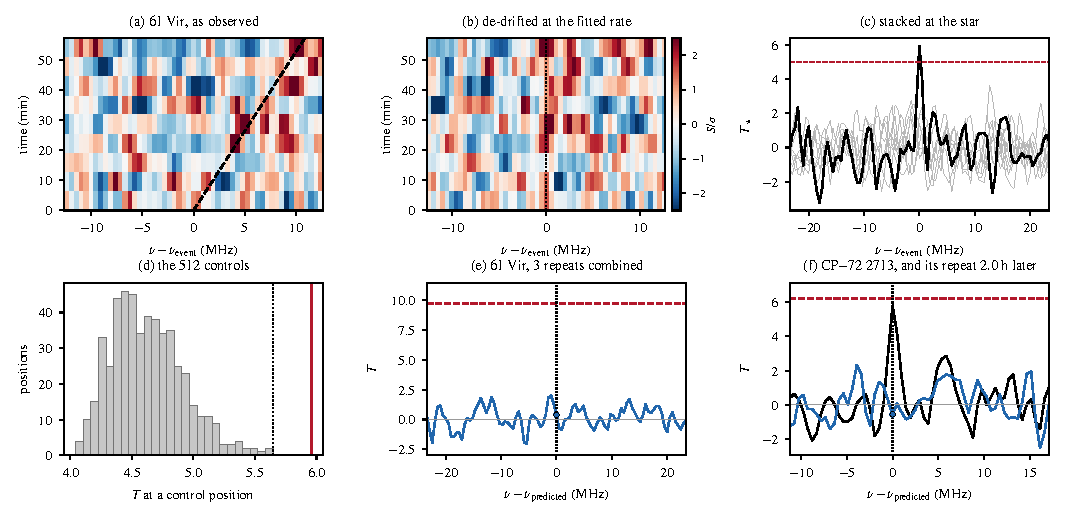
\includegraphics[width=\textwidth]{figures/event_crossings.pdf}
\caption{\textbf{The two crossings that lead their own control fields, and
why neither is a confirmed signal.} Frequencies are in the star's rest frame.
\emph{(a)}~The dynamic spectrum at \EvAStar's position around the crossing at
\RqFreqSx\,GHz, observed \EvADate, with the fitted drift of
\EvADrift\,Hz\,s$^{-1}$ as the dashed track; the \EvANInt{} integrations are
binned into \EvANBin{} and plotted in units of each bin's noise. At
\EvAFlux$\pm$\EvAFluxErr\,mJy against \EvARmsInt\,mJy per integration the
carrier is \EvAPerIntSig{} standard deviations in any one of them, and exists
only in the coherent stack of all \EvADwellMin{} minutes on source.
\emph{(b)}~The same rows shifted by that drift, which carries the carrier
\EvADriftChan{} channels of \EvAChanwkHz\,kHz across the observation.
\emph{(c)}~The de-drifted stack at the star (black) and at the
\RcNRetCtrl{} control positions with retained dynamic spectra (grey), in
units of its own noise; dashed, the trigger. \emph{(d)}~The same statistic at
each of the \NCtrl{} rank-screen control positions: the star (solid) against
the highest control (dotted). \emph{(e)}~The \EvANRep{} other blocks covering
that cell, combined, with zero at the predicted channel, which the frame
transport moves between epochs. Dashed, the $T_{\rm pers}=\EvATPers$ a
carrier persisting at the discovery flux would have given; circled, the
$T_{\rm rep}=\EvATRep$ read there at the carried drift, which excludes
anything above \RcSxFive{} of that flux. \emph{(f)}~The second event,
\EvBStar{} at \RqFreqCp\,GHz: its discovery stack (black) and the same cell
\EvBDeepH\,hours later in a block \EvBDeepRatio{} times deeper (blue), with
the same two marks at $T_{\rm pers}=\EvBDeepTPers$ and, in that one block,
$T_{\rm rep}=\EvBDeepTObs$ --- not the combination over all \ZdCpNRep{}
covering blocks that Table~\ref{tab:cand} prints. Panels~(e) and~(f) read one
channel at one drift, so each excludes only a carrier whose stellar-frame
frequency moved by less than $\pm\RqDispSx$ and $\pm\RqDispCp$\,km\,s$^{-1}$
between the epochs compared. The two events imply isotropic-equivalent powers
of $\EvAEirp\times10^{\EvAEirpExp}$\,W at \EvADistPc\,pc and
$\EvBEirp\times10^{\EvBEirpExp}$\,W at \EvBDistPc\,pc.}
\label{fig:event}
\end{figure*}

\begin{table}
\centering
\caption{\textbf{Can two crossings be one carrier?} Every pair of crossings
toward one star, in two execution blocks, within
\WdHalfKms\,km\,s$^{-1}$ of each other in the star's frame; stars are
identified by position, so the two archival-tail crossings of \TjDeepStar{}
pair with its catalogued ones. $\Delta\nu$ is the stellar-frame offset and
$\dot\nu_1$, $\dot\nu_2$ the drifts fitted independently in the two blocks.
A transmitter at constant line-of-sight acceleration would put the pair at
$\Delta\nu=\frac{1}{2}(\dot\nu_1+\dot\nu_2)\Delta t$; the last column gives
how far the pair is from that, in units of the drift grid's own resolution
carried over $\Delta t$. Italic entries are pairs for which that resolution
exceeds the window searched, so the comparison has no power and only the
agreement of the pairs' number with chance bears on them. The last row is the
control: the one pair whose two members this test accepts as a single
emitter, a molecular line recovered at one stellar-frame frequency in two
blocks.}
\label{tab:pairs}
\scriptsize
%% GENERATED by pairs_v415.py -- do not hand-edit.
\begin{tabular}{@{}l@{~}l@{~}r@{~}r@{~}r@{~}r@{~}r@{}}
\hline
Star & blocks & $\Delta t$ & $\dot\nu_1$ & $\dot\nu_2$ & $\Delta\nu$ & miss \\
 & & (d) & \multicolumn{2}{c}{(Hz\,s$^{-1}$)} & (MHz) & ($\sigma$) \\
\hline
61~Vir & X822/X82f & 3.00 & $+1052$ & $+3182$ & $+755.4$ & 16 \\
ALMA~J1537$-$3319 & X10359/X398 & 123 & $-2023$ & $+2373$ & $+223.5$ & 3.2 \\
AU~Mic & X1838/X319 & 310 & $+1419$ & $+2627$ & $-159.0$ & \emph{28} \\
HD~14055 & X2b2ee/X2c3bb & 0.09 & $-2426$ & $+4184$ & $+825.2$ & 2448 \\
 & X24be0/Xd46 & 1.92 & $+1104$ & $-3857$ & $+63.0$ & 42 \\
 & X2c3bb/X3835 & 2.00 & $+4184$ & $+1769$ & $-514.6$ & 143 \\
 & X2b2ee/X3835 & 2.09 & $-2426$ & $+1769$ & $+310.6$ & 49 \\
 & X3835/Xd526 & 607 & $+1769$ & $-2589$ & $-555.5$ & \emph{8.9} \\
 & X2b2ee/Xd526 & 609 & $-2426$ & $-2589$ & $-244.9$ & \emph{56} \\
 & X3835/X25c5e & 649 & $+1769$ & $+2584$ & $+423.3$ & \emph{49} \\
 & X2c3bb/X25c5e & 651 & $+4184$ & $+2584$ & $-91.3$ & \emph{76} \\
 & X2b2ee/X25c5e & 651 & $-2426$ & $+2584$ & $+733.8$ & \emph{1.5} \\
$\beta$~Pic & X3a90/Xa9df & 1.02 & $-1625$ & $-692$ & $+85.5$ & 132 \\
\hline
HD~285968 & X108f/X5b4e & 4.99 & $-49$ & $-48$ & $-0.002$ & 0.9 \\
\hline
\end{tabular}

\end{table}

\begin{table}
\centering
\caption{\textbf{The two events of Fig.~\ref{fig:event}}, the crossings whose
stellar statistic exceeds all \NCtrl{} control positions of their own window.
Repeat epochs measured are the blocks at which the predicted stellar-frame
cell was read; the indented rows give how many of those lie in the primary
census and how many census blocks cover the frequency at all, the remainder
coming from the archival extension.
$T_{\rm rep}$ combines every repeat epoch by inverse variance at the carried
drift: it is one cell and one trial, so it may be negative, and it is the
quantity $T_{\rm pers}$ is compared against. The indented readings beneath it
are the largest single epoch at that drift and the largest over every drift
trial, each a maximum and so positive on average whatever is there; the
single-epoch reading in the deepest block is the one Fig.~\ref{fig:event}(f)
marks, and it is not the combination. The exclusion is given as the fraction
of the discovery amplitude $S$ still ruled out at the trigger,
$(T_{\rm rep}+5)/T_{\rm pers}$. The significance at which the two readings of
one amplitude disagree saturates at $T_\star$ when the repeat coverage is
deep: over the \RqSatN{} crossings whose $T_{\rm pers}$ exceeds their own
$T_\star$ tenfold the ratio of the two is \RqSatRatioLo{} to
\RqSatRatioHi, so for \RqSatStar{} it returns \RqSatExcl{} against that row's
$T_\star=\RqSatTStar$. It restates the discovery significance rather than the
repeat, and is therefore not quoted. The displacement permitted
is half a channel in the star's frame, which is the interval the reading
covers, and beneath it the line-of-sight velocity a transmitter in a circular
orbit at 1\,au would acquire over the interval to the nearest covering block.
The last row but one is the chance $\Phi(T_{\rm pers}-5)$ that a carrier
persisting at $S$, and then at the trigger amplitude $5S/T_\star$, would have
satisfied the criterion at all.}
\label{tab:cand}
\footnotesize
%% GENERATED by recur_v411.py -- do not hand-edit.
\begin{tabular}{@{}>{\raggedright\arraybackslash}p{0.49\columnwidth}@{~~}r@{~~}r@{}}
\hline
 & 61 Vir & CP$-$72 2713 \\
\hline
Frequency, stellar frame (GHz) & 346.323236 & 344.296455 \\
\quad as delivered, topocentric & 346.313811 & 344.269746 \\
Channel width (kHz) & 488.28 & 488.28 \\
Drift rate (Hz\,s$^{-1}$) & $+3182$ & $-2056$ \\
$T_\star$ & 5.958 & 5.809 \\
Highest control $T$ & 5.65 & 5.68 \\
Flux density (mJy) & 118.8 $\pm$ 19.9 & 11.3 $\pm$ 2.0 \\
Peak-channel EIRP (W) & $5.1 \times 10^{14}$ & $8.9 \times 10^{14}$ \\
Repeat epochs measured & 3 & 5 \\
\quad in the primary census & 3 & 1 \\
\quad census blocks covering $\nu$ & 4 & 1 \\
Observed & 2017 May 20 & 2022 Oct 2 \\
Nearest covering epoch & 2017 May 19 & 2022 Oct 2 \\
\quad separation (h) & $-1.97$ & $+2.05$ \\
\quad covering epochs more than a day away & 2 & 4 \\
Longest baseline (d) & 3 & 2 \\
$T$ expected if persistent, $T_{\rm pers}$ & 9.70 & 6.30 \\
$T$ measured, matched drift, $T_{\rm rep}$ & +0.39 & -0.82 \\
\quad largest single epoch & +1.65 & +0.96 \\
\quad maximised over every drift & 2.71 & 3.60 \\
Amplitude still excluded, $(T_{\rm rep}+5)/T_{\rm pers}$ & 0.56 $S$ & 0.66 $S$ \\
Displacement permitted (km\,s$^{-1}$) & $\pm$0.211 & $\pm$0.213 \\
\quad a transmitter at 1\,au would move & 0.042 & 0.044 \\
Recovery chance if persistent, at $S$ / at $5\sigma$ & 1.00 / 1.00 & 0.90 / 0.66 \\
Disposition & not confirmed & not confirmed \\
\hline
\end{tabular}

\end{table}

\begin{table*}
\centering
\caption{\textbf{The threshold crossings of the reserved hold-out}, searched
with the same frozen pipeline and disposed of by the same tests as the
census. $\Delta v_\star$ is the offset from the nearest masked transition in
the star's own frame and $n_{\rm rep}$ the number of covering repeat blocks;
$T_{\rm pers}$ and $T_{\rm rep}$ are as in Table~\ref{tab:ledger}. The one
crossing that is present again is a carbon monoxide line.}
\label{tab:holdout}
\scriptsize
%% GENERATED by holdout_v412.py -- do not hand-edit.
\begin{tabular}{@{}l@{~}l@{~}r@{~}r@{~}l@{~}r@{~~}r@{~}r@{~}r@{~}l@{}}
\hline
Star & block & $\nu_{\rm topo}$ (GHz) & $T_\star$ & line & $\Delta v_\star$ & $n_{\rm rep}$ & $T_{\rm pers}$ & $T_{\rm rep}$ & disposition \\
\hline
HD~285968 & Xdaef5a\_Xdd9b & 230.5081 & 8.642 & CO($2$--$1$) & +8.7 & 4 & 11.6 & +6.71 & attributed; present again \\
HD~14055 & X107376c\_X6126 & 330.7123 & 5.513 & $^{13}$CO($3$--$2$) & +112.6 & 30 & 312.0 & +0.56 & unattributed; does not recur \\
TRAPPIST$-$1 & Xd0e450\_X259b & 346.2454 & 5.326 & SO($9_{8}$--$8_{7}$) & -306.6 & 5 & 11.1 & -0.32 & unattributed; does not recur \\
HD~172555 & X107fa96\_X1300f & 344.6066 & 5.144 & SO($8_{8}$--$7_{7}$) & +251.3 & --- & --- & --- & unattributed; no repeat coverage \\
HD~285968 & Xdb4b9a\_Xa7c & 229.9129 & 5.106 & CO($2$--$1$) & -768.0 & 4 & 11.2 & +0.21 & unattributed; does not recur \\
HR~1010 & Xc6b674\_X23f2 & 346.2301 & 5.044 & SO($9_{8}$--$8_{7}$) & -238.7 & 7 & 25.9 & -0.80 & unattributed; does not recur \\
HD~10647 & Xff99e1\_X9cdf & 345.7059 & 5.017 & SO($2_{3}$--$2_{1}$) & +37.1 & 13 & 142.1 & -0.93 & unattributed; does not recur \\
HD~170773 & Xff294f\_X1fb & 345.5597 & 5.001 & SO($2_{3}$--$2_{1}$) & -113.8 & 4 & 59.3 & +1.45 & unattributed; does not recur \\
\hline
\end{tabular}

\end{table*}

%% tab:ledger MOVED to Appendix D (sections/app_J_falsealarm.tex): a
%% full-width 56-row table* worth 0.72 pp of the main text.  Sec. 5.3 and
%% Sec. 5.6 carry the counts and cite it.



%% fig:chain MOVED to sections/04_method.tex, Sec. 4.2, where it is first
%% cited (referee 2, minor 3).  Sec. 5 cites it at the crossing census.

%% ---------------------------------------------------------------------
%% REQUEST (results owner -> numbers owner).  Eight macros this file uses
%% that the frozen layer does not yet define, all on the adopted
%% trigger-plus-spatial-screen criterion (EirpNinetyMultA = 5.70):
%%   \EirpNinetyWinMedA                      median Class A window, W
%%   \EirpNinetySysLoA \EirpNinetySysMedA \EirpNinetySysHiA
%%                                           per system, best window, W
%%   \EirpNinetyBarnLo \EirpNinetyBarnHi     Barnard's Star, W
%%   \EirpNinetyWolfLo \EirpNinetyWolfHi     Wolf 359, W
%% The \Promote* family (\PromoteMedA, \PromoteSysMedA, ...) is the same
%% quantity on the superseded localisation criterion and is cited nowhere
%% in this file; it is still cited in 03_sample.tex and 07_conclusions.tex,
%% which must move to the names above or the paper will carry two
%% sensitivities again.  \EirpBarnLo/\EirpBarnHi/\EirpWolfLo/\EirpWolfHi
%% are nominal triggers and are no longer quoted here.
%%
%% REQUEST (results owner -> numbers owner).  tab_ledger_v403 must drop
%% nine columns: both visibility-fit epoch groups (Re/sigma, Im/sigma,
%% ctrl, twice), the epoch displacement D, the off-channel column "off",
%% and the "scr" rank flag, whose result is carried by the disposition
%% code.  Eight columns remain: star, block, band, nu, T_star, line, dv,
%% disposition.  \LedgerLegend is replaced by the caption above, so the
%% legend macro is no longer referenced.
%%
%% REQUEST (results owner -> numbers owner).  tab_maskladder.tex now has a
%% home as Table tab:maskladder in this file.  Its fourth column header
%% reads "rank-flagged", a phrase this manuscript has used in both senses;
%% please rename it to "outrank all controls" so the header cannot be read
%% as its own opposite.  The caption states the meaning meanwhile.
%%
%% REQUEST (results owner -> figures owner).  fig:chain MUST BE RE-EMITTED
%% AT SINGLE-COLUMN GEOMETRY.  It is now a \begin{figure} at \columnwidth,
%% not a figure* at 0.98\textwidth, because the section measures 6.0 pp as
%% three full-width floats and 5.0 pp with this one in a column -- the
%% overage was float packing, not words.  chain_v403.pdf is still drawn for
%% full width, so its labels are currently at about half their intended
%% size: PLEASE RE-EMIT FOR ONE COLUMN.  A six-step vertical chain reads
%% better in a column than across a page, so this is the right geometry
%% for it, but the caption, the placement and the artwork must agree and
%% today only two of the three do.  If re-emission is refused, revert this
%% float to figure*/0.98\textwidth and the section is 6.0 pp.
%%
%% REQUEST (results owner -> figures owner).  fig:bpiccontrol.
%%  - GEOMETRY CONFIRMED SINGLE COLUMN.  bpic_control.pdf is 237.6 x 280.7 pt,
%%    i.e. one column wide with the two panels stacked vertically, and the
%%    float is \columnwidth in a \begin{figure}.  Caption and placement
%%    agree; no re-emission at full width is wanted.  Panel (b) gets the
%%    full column width this way, which is what it needs.
%%  - COUNTS I WOULD NOT INVENT.  \NStageOneBpicEb (9) counts the blocks in
%%    which the star outranks every control, so it cannot also count the
%%    points drawn: the ring-wins block is by definition not one of the 9.
%%    The caption therefore says "the 9 ... and one further block" rather
%%    than giving a total.  Four macros would let it say what is drawn:
%%      \BpicPanelNCo     beta Pic CO points in panel (b)        (10)
%%      \BpicPanelNOther  other crossings drawn in grey          (39)
%%      \BpicDvCoLo \BpicDvCoHi   |dv| range of the CO crossings (12-29)
%%      \BpicDvCsLo \BpicDvCsHi   |dv| of the two CS(5-4) crossings
%%    \BpicDvLo/\BpicDvHi existed earlier today and have since been retired.
%%  - COUNTEREXAMPLE NUMBERS, requested and still absent: the ring maximum
%%    (14.13), the stellar statistic (9.68) and the number of the \NCtrl
%%    controls above the star (6) in the ring-wins block.  When they exist
%%    the caption should name that block instead of gesturing at it.
%%
%% REQUEST (results owner -> integrator).  Labels and floats deleted from
%% this file, with the files that still reference them:
%%   sec:linecost     -> sec:bpicval   (06_discussion, app_F, app_I, app_K)
%%   sec:repairedstat -> app:v409      (08_backmatter, app_A, app_M)
%%   eq:tunif         no longer defined anywhere (app_L cites it)
%%   tab:crossdelta   float deleted with the revision-history material;
%%                    app_M_repaired.tex still cites it
%%   tab:clustv409    float deleted; nothing else cites it
%%   fig:ledgervis    no longer cited (float lives in app_K)
%%   tab:hosts        no longer cited from here
%%   app:etacrvrecur  no longer cited from here (app_M still cites it)
%% ---------------------------------------------------------------------
